\chapter[Trabajos relacionados ]{Trabajos relacionados }\label{ch:capitulo2}

En el área del reconocimiento de patrones, visión por computadora es un área que posee muchos estudios~\cite{Andreopoulos2013}. Es por esto que en este capítulo pasaremos a revisar diversas técnicas y algoritmos. Una de las ideas básicas de estos algoritmos es que sean capaces de recibir una imagen como entrada y crear una representación que describa los objetos que estén presentes en dicha imagen. Este capítulo comprende el detalle de las técnicas de detección y reconocimiento, tanto para objetos como para expresiones faciales. Si bien esta área es extensa, trataremos de abarcar aquellas investigaciones que sean relevantes, y nos ayuden a crear las bases para nuestro trabajo.

% SECCION DE DETECCION
\section{Detección y reconocimiento}
La detección de objetos es una tarea ardua que ha sido estudiada durante décadas, esto se puede ver en el estudio que resume 50 años de investigación relacionada con el reconocimiento de objetos~\cite{Andreopoulos2013} lo que nos da una gran visión de lo que se a realizado en esta área, este estudio nos entrega una mirada especialista y nos plantea ¿cuál es el fin de detectar objetos? Lo que nos llama mucho la atención, y si lo pensamos detenidamente, podemos plantear lo siguiente, detectando objetos en una imagen o en una secuencia de imágenes buscamos utilizar aquello que en dichas imágenes es único y las describa, así el color de ojos, la forma de hablar, o la forma de la cara de una persona la diferencia de otra, por ejemplo, eso nos da el puntapié inicial para describir lo que en esa imagen se está viendo, si bien el objetivo de detectar objetos es lograr obtener una representación fiel de éste, se busca encontrar una manera de representar o modelar las características únicas de una imagen con el fin de poder clasificarla para posteriormente ser utilizada para tomar decisiones que utilicen algún programa o aplicación.

En cuanto al reconocimiento de objetos se han realizado estudios en dos contextos: objetos rígidos en 2D y 3D\@. El objetivo principal del \textit{reconocimiento de objetos}, es poder clasificar de forma correcta las clases que se están observando. A modo de ejemplo, en una escena donde hay siete perros y tres gatos, el objetivo del algoritmo que se utilice es que identifique, con el menor error posible, los siete perros que hay en una escena como perros, y de igual manera para los tres gatos.

Para la detección y reconocimiento de rostros también existen investigaciones que proponen excelentes mecanismos para realizar estas tareas, algunas de estas propuestas se presentan en la Sección~\ref{subsec:expre}, ahora bien, detectar y reconocer rostros es una tarea más que estudiada, por lo que surgen preguntas como ¿qué pasa con los sentimientos que expresa un rostro?, ¿podrá ser capaz un computador saber mi estado de ánimo solo viendo mi cara? este tema abre otro capítulo de discusión y también se presentan en este Capítulo estudios que comienzan a abarcar este tópico tan interesante, interesante para nuestro trabajo, ya que tocaremos este punto en nuestra propuesta y saber que se ha realizado en este tópico en particular es de gran ayuda.

En otras áreas de la detección y reconocimiento, tenemos el reconocimiento óptico de caracteres el cual juega un rol fundamental en la tarea de digitalización de libros, ya que al generarse tanta información escrita y de distintas formas, poder crear un sistema que lo haga automáticamente detectando ciertos patrones en los datos utilizados, en este caso caracteres alfanuméricos. Esto implica un importante ahorro de recursos humanos y un aumento de la productividad, al mismo tiempo que se mantiene, o hasta se mejora, la calidad de muchos servicios.

\subsection{Modelo}
\label{subsec:modelo}

\begin{definition}[Modelo]
Un modelo es una abstracción teórica del mundo real, que nos permite representar la información de forma simplificada con el objetivo de realizar predicciones con los datos necesarios.
\end{definition}

Estos modelos permiten encontrar \textit{igualdades o similitudes} en los datos. Más en concreto, se suele entrenar un modelo con un conjunto de datos que representan una clase, para luego usar esta representación para predecir nuevos datos de entrada. En cuanto a la detección y reconocimiento de objetos, se utilizan modelos llamados descriptores, los cuales son algoritmos que extraen características más representativas de una imagen.

\begin{definition}[Modelos estadísticos]\label{def:mod_est}
Un modelo estadístico es una ecuación matemática que reproduce los fenómenos que observamos de la forma más exacta posible. Para ello tiene en cuenta los datos suministrados y la influencia que el azar tiene en estas observaciones. Esto nos permite tener una abstracción más exacta de sucesos cotidianos.
\end{definition}
\begin{definition}[Descriptor]\label{def:desc}
Un descriptor no es más que un conjunto de características. Es decir, un especie de modelo que representa las características extraídas en forma vectorial.
\end{definition}


\subsection{Modelos de detección y reconocimiento de objetos}
Torres-Méndez et al.~\cite{trsi2000}, presenta un modelo de reconocimiento de objetos, que es invariante a la posición de éste, a su rotación y su escala. Se presenta un algoritmo que en primera instancia, pre-procesa los datos, con el fin de normalizar los momentos de inercia que posee el objeto, extrayendo así las características topológicas del objeto. En una segunda fase, el reconocimiento es logrado usando el algoritmo \textit{Holographic Nearest-Neighbor} (\textit{HNN}). El principal motivo por el cual se utiliza este algoritmo es su rapidez~\cite{trsi2000}, ya que a diferencia de otras arquitecturas de redes neuronales, este algoritmo es bastante rápido según Torres-Méndez et al.~\cite{trsi2000}. En general, HNN posee un mejor desempeño al momento de reconocer, a diferencia de técnicas como \textit{Nearest-Neightbor} (\textit{NN}). El algoritmo HNN es similar al NN, este último está basado en la idea de utilizar la mínima distancia euclidiana entre el vector de entrada (modelo del objeto que se intenta reconocer) y todos los vectores de entrenamiento (el conjunto de modelos de los objetos de entrenamiento). Además, para evitar la predominancia de algunos sub-grupos de características, el algoritmo NN normaliza las características. Esta normalización consiste en extraer el promedio de los vectores de características y dividirlo por la desviación estándar de cada una de las características presentes en el conjunto de datos de entrenamiento.

Amit~\cite{Amit2002}, presenta técnicas como: \textit{Searching Correspondence Space}, el cual realiza una búsqueda sistemática, para el conjunto de características locales de la imagen. En este caso los emparejamientos deben satisfacer ciertas restricciones. Restricciones únicas implican una relación directa entre las características del modelo y las características de la imagen. Restricciones binarias implican la relación entre un par de características del modelo y de un par de características de la imagen. Diversas técnicas basadas en heurísticas de árboles se emplean para encontrar los diversos emparejamientos, con el fin de encontrar el emparejamiento óptimo de estas características. A su vez, se presentan varios modelos para reconocimiento de objetos, muchos de ellos utilizados por estudios realizados en esta área. Por ejemplo, \textit{Deformable-Template Models} representa las características de un objeto, utilizando un modelo estadístico (ver Sección~\ref{subsec:modelo}), el cual describe la variabilidad que posee una instancia de un objeto en términos de una probabilidad a priori. Además, una representación  estadística de la imagen, entrega una particular deformación de la porción del objeto analizado. La combinación de ésta representación y la probabilidad priori, definen una distribución posterior de la deformación que posee la imagen.

Lowe~\cite{sift2004} presenta un método para la extracción de características invariantes de una imagen que son utilizadas para hacer una comparación entre diferentes vistas o escenas de un objeto. Las características son invariantes a la escala de la imagen y la rotación que esta pueda presentar. Los descriptores se representan con la dirección y el gradiente que poseen los puntos de interés encontrados en etapas previas, luego se preprocesan los datos con una función de peso gaussiana, la cual asigna un peso a cada uno de los puntos. El propósito de este filtro es evitar que las muestras sufran variaciones.

En Bernstein~\cite{statistical2005}, se propone un modelo denso y con un rendimiento que otorga una tasa de clasificación alta, este modelo consiste en una mejora a los modelos \textit{Sparse}, descritos por Amit~\cite{Amit2002}. este modelo usa una mezcla de partes que definen, a un nivel medio, características locales basándose en orientaciones binarias en los bordes de los datos de entrada. Este estudio probó su modelo en un conjunto acotado de caracteres escritos a mano, además, se probó en y entreno para poder detectar distintos lados de automóviles.

Bay et al.~\cite{surf2008} presenta un detector y descriptor que es invariante a las rotaciones, llamado \textit{Speeded-Up Robust Feature} (\textit{SURF}). SURF utiliza un descriptor basado en distribuciones. Para SURF la creación de un descriptor debe ser único e invariante al ruido, para esto cada descriptor define una distribución de intensidad de los puntos adyacentes al punto de interés, similar a lo que se postula en Lowe~\cite{sift2004}, pero con la diferencia que no se utiliza el gradiente sino que una distribución de primer orden basado en los \textit{wavelet} de Haar.

Felzenszwalb et al.~\cite{Felzenszwalb2010} presenta un modelo basado en partes,  el cual utiliza varias partes de la imagen con el fin de determinar si existe un objeto de interés en ella. En este trabajo se busca optimizar el detector de Dalal-Triggs el que utiliza \textit{Histogram of Oriented Gradients} (\textit{HOG})~\cite{hog2005} (ver Sección~\ref{subsec:hog}). Éste tiene como principal objetivo obtener características específicas del objeto mediante la dirección de los gradientes o bordes, este proceso es implementado de la siguiente forma: Se divide la imagen en pequeñas porciones, llamadas celdas, las cuales generan otros histogramas de gradientes o bordes por cada pixel dentro de esta celda, combinando estos histogramas se obtiene la representación del descriptor. La mejora realizada sobre este método es que en paralelo se computa una función que maximiza los puntos obtenidos por HOG, lo cual permite capturar más características en el mismo rango de muestreo, este estudio será analizado con mayor detalle en el Capítulo~\ref{ch:capitulo4}.

Choi et al.~\cite{treebased2012} proponen un modelo basado en el contexto, el cual maneja distintas combinaciones o locaciones de objetos que guía un detector el cual produce una interpretación semántica de la imagen que se está analizando. El objetivo de este trabajo es poder detectar múltiples categorías de objetos dentro de una misma escena. Por lo cual su modelo utiliza características globales dependientes entre las categorías de los objetos y las salidas locales de los descriptores utilizados.

\subsection{Modelos de detección y reconocimiento de expresiones}\label{subsec:expre}
Comúnmente existen dos enfoques para la extracción de características en el rostro: Basados en características geométricas y basados en apariencia. El primer tipo de métodos utiliza relaciones entre distintas partes del rostro para crear los descriptores. Mientras que el último método utiliza filtros que crean características, generales o en una área del rostro en específico, con el fin de extraer los cambios de apariencia en la imagen del rostro.

Hsu et al.~\cite{Hsu2002} presentan un algoritmo de detección de rostros que trabaja con imágenes a color, tomando en cuenta distintas condiciones de luminosidad, así como fondos complejos. Ellos definen que los rostros humanos juegan un importante rol en las aplicaciones actuales. Dicho algoritmo funciona de la siguiente manera. Primero, el algoritmo detecta las regiones donde está presente la piel, y luego genera un rostro candidato basado en la disposición espacial de estos parches cutáneos. Finalmente, el algoritmo construye los ojos, boca y el mapa de los contornos, para verificar cada rostro candidato. En concreto, el algoritmo primero estima y corrige el sesgo de color basado en una técnica de compensación de la iluminación. La corrección realizada a los componentes de los colores rojo, verde y azul son transformadas no linealmente a otro espacio de color. Los píxeles de los tonos de de la piel son detectados usando un modelo de piel elíptico en el espacio transformado. La elipse paramétrica corresponde a los contornos de constantes de la distancia de Mahalanobis bajo el supuesto de una distribución de Gauss para el color del tono de la piel. El tamaño de un rostro candidato puede variar desde lo $13 \times 13$ píxeles hasta cerca de tres cuartos del tamaño de la imagen de entrada. El detector de características faciales rechaza todos los candidatos de rostros que no contengan características tales como los ojos, la boca o contornos del rostro.

Ahonen et al.~\cite{ahonen2006} presentan una representación eficiente del rostro, basándose en las características de las texturas extraídas por \textit{Local Binary Pattern} (\textit{LBP}). En primera instancia, la imagen es dividida en múltiples regiones donde es utilizado LBP para extraer las características locales de cada región, para luego ser representadas en un vector que contiene todas las regiones del rostro, el cual es utilizado como descriptor. La Figura~\ref{fig:lbp} muestra como es el proceso básico que realiza \textit{LBP}. Este operador asigna una etiqueta a cada píxel de una imagen por un umbral que corresponde al valor del pixel del centro de un vecindario de $3 \times 3$ y teniendo en cuenta el resultado como un número binario. Entonces, el histograma de las etiquetas puede ser utilizado como un descriptor de textura.

\begin{figure}[tb]
 \centering
  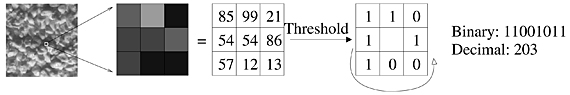
\includegraphics[width=1\textwidth]{Figuras/lbp.jpg}
  \caption[Operación básica de LBP]{Operación básica de LBP~\cite{ahonen2006}.}
  \label{fig:lbp}
\end{figure}

Ramírez et al.~\cite{ldnp2013} presenta un nuevo descriptor de características locales, llamado \textit{Local Directional Number Pattern} (\textit{LDN}), para el reconocimiento de rostro y expresiones. Este estudio comenta que la eficiencia de un descriptor depende de su representación y la facilidad de extracción del rostro. Idealmente un descriptor debería tener una alta varianza con clases muy distintas (diferentes personas o expresiones), por otra parte si las clases son semejantes (misma persona o expresión), su varianza debería ser mínima. La Figura~\ref{fig:ldn} muestra el proceso base de este algoritmo (\textit{LDN}). LDN codifica la estructura de un vecindario local mediante el análisis de su información direccional. En consecuencia, calculamos las respuestas de borde en el vecindario, en ocho direcciones diferentes. Luego, desde todas las direcciones, se eligen las mejores direcciones positivas y negativas, para producir un descriptor significativo para diferentes texturas con patrones estructurales similares. Este enfoque permite distinguir los cambios de intensidad (por ejemplo, de brillante a oscuro y viceversa) en la textura, que de otra manera se perdió.

\begin{figure}[tb]
 \centering
  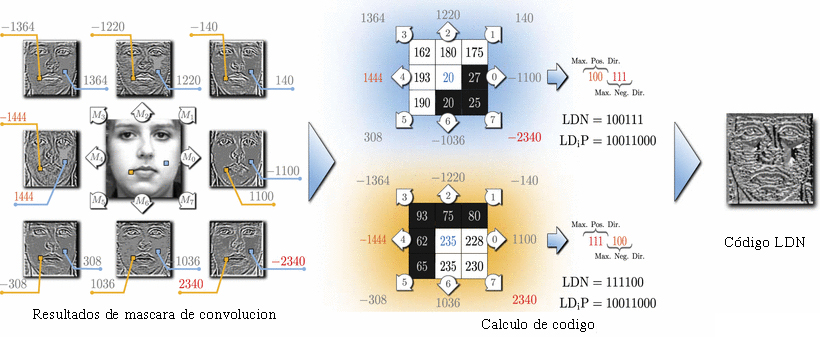
\includegraphics[width=1\textwidth]{Figuras/ldn.jpg}
  \caption[Calculo de LDN]{Calculo de LDN~\cite{ldnp2013}.}
  \label{fig:ldn}
\end{figure}

Zhu y Ramanan~\cite{Zhu2012} presentan un modelo unificado para detección de rostros, estimación de pose y contornos, este modelo está basado en una mezcla de árboles que comparten un conjunto de partes $V$. Se modela cada marca del rostro como una parte y se utiliza un mezcla global para capturar los cambios topológicos de acuerdo al punto de vista. En la Figura~\ref{fig:m-view} se observan las mezclas de los puntos de vista.

\begin{figure}[tb]
 \centering
  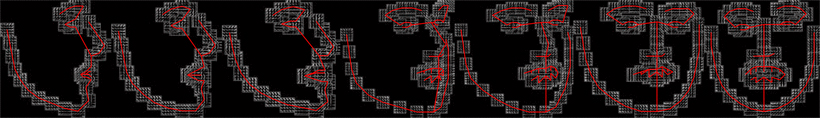
\includegraphics[width=1\textwidth]{Figuras/viewpoints.jpg}
  \caption[Puntos de vista de un rostro]{El modelo de mezcla-de-árboles codifica cambios topológicos debido al punto de vista. Las líneas rojas indican las descendencias entre pares de piezas; notar no hay bucles cerrados, manteniendo la propiedad de árbol. Todos los árboles hacen uso de un fondo común y compartida de Plantillas de partes, lo que hace que el aprendizaje y la inferencia sean eficiente~\cite{Zhu2012}.}
  \label{fig:m-view}
\end{figure}

Para que el algoritmo pueda aprender a clasificar, se utiliza un escenario completamente supervisado, donde se entregan como datos de entrada imágenes que contienen rostros (positivas) e imágenes sin presencia de rostros (negativas). Para poder clasificar se utiliza el algoritmo \textit{Chow-Liu}~\cite{Chow1968} con el objetivo de encontrar el máximo \textit{likelihood} para la estructura del árbol que mejor explique la posición de las marcas para una mezcla dada, asumiendo que todas las marcas del rostro presentan una distribución Gausiana.

\subsection{Resumen}
Este capítulo detalla varios estudios realizados previamente tanto en el área de la detección y reconocimiento de objetos, como en la detección y reconocimiento de rostros, lo cual nos permite tanto tener una idea de como trabajar sobre objetos y rostros. Nos enfocaremos en aquellos estudios los cuales utilizan partes de las imágenes para representar con más detalle los elementos que éstas puedan tener. Trabajos realizados por D. Ramanan y su grupo de trabajo serán de vital importancia para nuestro desarrollo puesto que lo realizado por él, es lo más cercano a lo que deseamos hacer para este estudio. Es así que los modelos basados en partes, más lo descriptores locales y el uso de técnicas de clasificación serán parte de las herramientas que utilizaremos en capítulos posteriores para ensamblar nuestro trabajo.


